% Options for packages loaded elsewhere
\PassOptionsToPackage{unicode}{hyperref}
\PassOptionsToPackage{hyphens}{url}
%
\documentclass[
]{article}
\usepackage{amsmath,amssymb}
\usepackage{lmodern}
\usepackage{iftex}
\ifPDFTeX
  \usepackage[T1]{fontenc}
  \usepackage[utf8]{inputenc}
  \usepackage{textcomp} % provide euro and other symbols
\else % if luatex or xetex
  \usepackage{unicode-math}
  \defaultfontfeatures{Scale=MatchLowercase}
  \defaultfontfeatures[\rmfamily]{Ligatures=TeX,Scale=1}
\fi
% Use upquote if available, for straight quotes in verbatim environments
\IfFileExists{upquote.sty}{\usepackage{upquote}}{}
\IfFileExists{microtype.sty}{% use microtype if available
  \usepackage[]{microtype}
  \UseMicrotypeSet[protrusion]{basicmath} % disable protrusion for tt fonts
}{}
\makeatletter
\@ifundefined{KOMAClassName}{% if non-KOMA class
  \IfFileExists{parskip.sty}{%
    \usepackage{parskip}
  }{% else
    \setlength{\parindent}{0pt}
    \setlength{\parskip}{6pt plus 2pt minus 1pt}}
}{% if KOMA class
  \KOMAoptions{parskip=half}}
\makeatother
\usepackage{xcolor}
\usepackage[margin=1in]{geometry}
\usepackage{color}
\usepackage{fancyvrb}
\newcommand{\VerbBar}{|}
\newcommand{\VERB}{\Verb[commandchars=\\\{\}]}
\DefineVerbatimEnvironment{Highlighting}{Verbatim}{commandchars=\\\{\}}
% Add ',fontsize=\small' for more characters per line
\usepackage{framed}
\definecolor{shadecolor}{RGB}{248,248,248}
\newenvironment{Shaded}{\begin{snugshade}}{\end{snugshade}}
\newcommand{\AlertTok}[1]{\textcolor[rgb]{0.94,0.16,0.16}{#1}}
\newcommand{\AnnotationTok}[1]{\textcolor[rgb]{0.56,0.35,0.01}{\textbf{\textit{#1}}}}
\newcommand{\AttributeTok}[1]{\textcolor[rgb]{0.77,0.63,0.00}{#1}}
\newcommand{\BaseNTok}[1]{\textcolor[rgb]{0.00,0.00,0.81}{#1}}
\newcommand{\BuiltInTok}[1]{#1}
\newcommand{\CharTok}[1]{\textcolor[rgb]{0.31,0.60,0.02}{#1}}
\newcommand{\CommentTok}[1]{\textcolor[rgb]{0.56,0.35,0.01}{\textit{#1}}}
\newcommand{\CommentVarTok}[1]{\textcolor[rgb]{0.56,0.35,0.01}{\textbf{\textit{#1}}}}
\newcommand{\ConstantTok}[1]{\textcolor[rgb]{0.00,0.00,0.00}{#1}}
\newcommand{\ControlFlowTok}[1]{\textcolor[rgb]{0.13,0.29,0.53}{\textbf{#1}}}
\newcommand{\DataTypeTok}[1]{\textcolor[rgb]{0.13,0.29,0.53}{#1}}
\newcommand{\DecValTok}[1]{\textcolor[rgb]{0.00,0.00,0.81}{#1}}
\newcommand{\DocumentationTok}[1]{\textcolor[rgb]{0.56,0.35,0.01}{\textbf{\textit{#1}}}}
\newcommand{\ErrorTok}[1]{\textcolor[rgb]{0.64,0.00,0.00}{\textbf{#1}}}
\newcommand{\ExtensionTok}[1]{#1}
\newcommand{\FloatTok}[1]{\textcolor[rgb]{0.00,0.00,0.81}{#1}}
\newcommand{\FunctionTok}[1]{\textcolor[rgb]{0.00,0.00,0.00}{#1}}
\newcommand{\ImportTok}[1]{#1}
\newcommand{\InformationTok}[1]{\textcolor[rgb]{0.56,0.35,0.01}{\textbf{\textit{#1}}}}
\newcommand{\KeywordTok}[1]{\textcolor[rgb]{0.13,0.29,0.53}{\textbf{#1}}}
\newcommand{\NormalTok}[1]{#1}
\newcommand{\OperatorTok}[1]{\textcolor[rgb]{0.81,0.36,0.00}{\textbf{#1}}}
\newcommand{\OtherTok}[1]{\textcolor[rgb]{0.56,0.35,0.01}{#1}}
\newcommand{\PreprocessorTok}[1]{\textcolor[rgb]{0.56,0.35,0.01}{\textit{#1}}}
\newcommand{\RegionMarkerTok}[1]{#1}
\newcommand{\SpecialCharTok}[1]{\textcolor[rgb]{0.00,0.00,0.00}{#1}}
\newcommand{\SpecialStringTok}[1]{\textcolor[rgb]{0.31,0.60,0.02}{#1}}
\newcommand{\StringTok}[1]{\textcolor[rgb]{0.31,0.60,0.02}{#1}}
\newcommand{\VariableTok}[1]{\textcolor[rgb]{0.00,0.00,0.00}{#1}}
\newcommand{\VerbatimStringTok}[1]{\textcolor[rgb]{0.31,0.60,0.02}{#1}}
\newcommand{\WarningTok}[1]{\textcolor[rgb]{0.56,0.35,0.01}{\textbf{\textit{#1}}}}
\usepackage{graphicx}
\makeatletter
\def\maxwidth{\ifdim\Gin@nat@width>\linewidth\linewidth\else\Gin@nat@width\fi}
\def\maxheight{\ifdim\Gin@nat@height>\textheight\textheight\else\Gin@nat@height\fi}
\makeatother
% Scale images if necessary, so that they will not overflow the page
% margins by default, and it is still possible to overwrite the defaults
% using explicit options in \includegraphics[width, height, ...]{}
\setkeys{Gin}{width=\maxwidth,height=\maxheight,keepaspectratio}
% Set default figure placement to htbp
\makeatletter
\def\fps@figure{htbp}
\makeatother
\setlength{\emergencystretch}{3em} % prevent overfull lines
\providecommand{\tightlist}{%
  \setlength{\itemsep}{0pt}\setlength{\parskip}{0pt}}
\setcounter{secnumdepth}{-\maxdimen} % remove section numbering
\ifLuaTeX
  \usepackage{selnolig}  % disable illegal ligatures
\fi
\IfFileExists{bookmark.sty}{\usepackage{bookmark}}{\usepackage{hyperref}}
\IfFileExists{xurl.sty}{\usepackage{xurl}}{} % add URL line breaks if available
\urlstyle{same} % disable monospaced font for URLs
\hypersetup{
  pdftitle={Data exploration and deterministic functions},
  pdfauthor={David Murillo},
  hidelinks,
  pdfcreator={LaTeX via pandoc}}

\title{Data exploration and deterministic functions}
\author{David Murillo}
\date{October 7, 2022}

\begin{document}
\maketitle

{
\setcounter{tocdepth}{2}
\tableofcontents
}
load packagues

\begin{Shaded}
\begin{Highlighting}[]
\FunctionTok{library}\NormalTok{(here)}
\end{Highlighting}
\end{Shaded}

\begin{verbatim}
## here() starts at C:/Users/DavidMurillo/OneDrive - University of Massachusetts/Umass/Classes/Fall2022/DataAna/environmental_data
\end{verbatim}

load data set

\begin{Shaded}
\begin{Highlighting}[]
\NormalTok{habitat }\OtherTok{\textless{}{-}} \FunctionTok{read.csv}\NormalTok{(}\FunctionTok{here}\NormalTok{(}\StringTok{"data"}\NormalTok{, }\StringTok{"hab.sta.csv"}\NormalTok{))}
\end{Highlighting}
\end{Shaded}

Examine histograms of the three terrain variables.

Plot histograms of the following terrain variables: elevation aspect
slope

\begin{Shaded}
\begin{Highlighting}[]
\FunctionTok{hist}\NormalTok{(habitat}\SpecialCharTok{$}\NormalTok{elev, }\AttributeTok{main =} \StringTok{"Histogram of elevation"}\NormalTok{,}
     \AttributeTok{xlab=} \StringTok{"Elevation"}\NormalTok{)}
\end{Highlighting}
\end{Shaded}

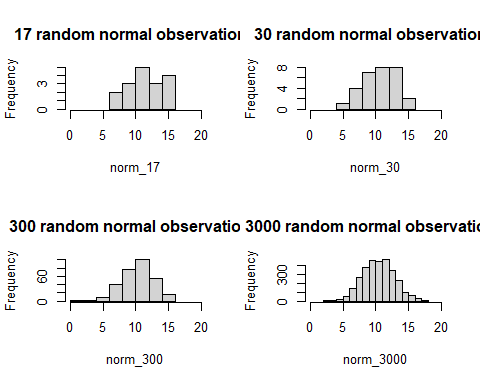
\includegraphics{Data_exploration_deterministic_functions_David_Murillo_files/figure-latex/unnamed-chunk-3-1.pdf}

\begin{Shaded}
\begin{Highlighting}[]
\FunctionTok{hist}\NormalTok{(habitat}\SpecialCharTok{$}\NormalTok{aspect, }\AttributeTok{main =} \StringTok{"Histogram of aspec"}\NormalTok{,}
     \AttributeTok{xlab=} \StringTok{"Aspec"}\NormalTok{)}
\end{Highlighting}
\end{Shaded}

\includegraphics{Data_exploration_deterministic_functions_David_Murillo_files/figure-latex/unnamed-chunk-3-2.pdf}

\begin{Shaded}
\begin{Highlighting}[]
\FunctionTok{hist}\NormalTok{(habitat}\SpecialCharTok{$}\NormalTok{slope, }\AttributeTok{main =} \StringTok{"Histogram of Slope"}\NormalTok{,}
     \AttributeTok{xlab=} \StringTok{"Slope"}\NormalTok{)}
\end{Highlighting}
\end{Shaded}

\includegraphics{Data_exploration_deterministic_functions_David_Murillo_files/figure-latex/unnamed-chunk-3-3.pdf}

\begin{enumerate}
\def\labelenumi{\arabic{enumi}.}
\tightlist
\item
  Create scatterplots of total basal area and the terrain variables
  (consult the metadata file to see which column(s) you need).
\end{enumerate}

Basal area should be on the y-axis.

Visually inspect the plots and fit a linear function to each of the
scatterplots using the parameterization functions provided above.

You'll need this fitted model for the assignment questions.

\begin{Shaded}
\begin{Highlighting}[]
\CommentTok{\# Calculates the value of y for a linear function, given the coordinates}
\CommentTok{\# of a known point (x1, y1) and the slope of the line.}
\NormalTok{line\_point\_slope }\OtherTok{=} \ControlFlowTok{function}\NormalTok{(x, x1, y1, slope)}
\NormalTok{\{}
\NormalTok{  get\_y\_intercept }\OtherTok{=} 
    \ControlFlowTok{function}\NormalTok{(x1, y1, slope) }
      \FunctionTok{return}\NormalTok{(}\SpecialCharTok{{-}}\NormalTok{(x1 }\SpecialCharTok{*}\NormalTok{ slope) }\SpecialCharTok{+}\NormalTok{ y1)}
  
\NormalTok{  linear }\OtherTok{=} 
    \ControlFlowTok{function}\NormalTok{(x, yint, slope) }
      \FunctionTok{return}\NormalTok{(yint }\SpecialCharTok{+}\NormalTok{ x }\SpecialCharTok{*}\NormalTok{ slope)}
  
  \FunctionTok{return}\NormalTok{(}\FunctionTok{linear}\NormalTok{(x, }\FunctionTok{get\_y\_intercept}\NormalTok{(x1, y1, slope), slope))}
\NormalTok{\}}
\end{Highlighting}
\end{Shaded}

\begin{Shaded}
\begin{Highlighting}[]
\FunctionTok{plot}\NormalTok{(habitat}\SpecialCharTok{$}\NormalTok{elev, habitat}\SpecialCharTok{$}\NormalTok{ba.tot)}
\FunctionTok{curve}\NormalTok{(}\FunctionTok{line\_point\_slope}\NormalTok{(x, }\AttributeTok{x1 =} \FloatTok{3.5}\NormalTok{, }\AttributeTok{y1 =} \FloatTok{1.25}\NormalTok{, }\AttributeTok{slope =} \FloatTok{0.4}\NormalTok{), }\AttributeTok{add =} \ConstantTok{TRUE}\NormalTok{)}
\end{Highlighting}
\end{Shaded}

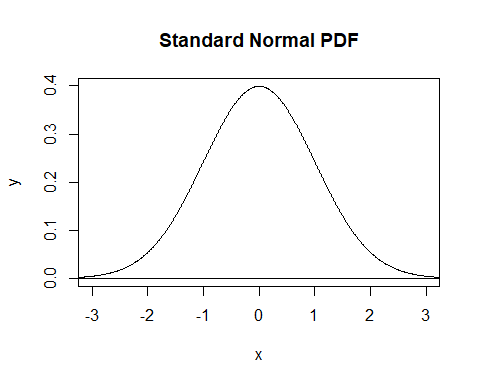
\includegraphics{Data_exploration_deterministic_functions_David_Murillo_files/figure-latex/unnamed-chunk-5-1.pdf}

\begin{Shaded}
\begin{Highlighting}[]
\FunctionTok{plot}\NormalTok{(habitat}\SpecialCharTok{$}\NormalTok{aspect, habitat}\SpecialCharTok{$}\NormalTok{ba.tot)}
\FunctionTok{curve}\NormalTok{(}\FunctionTok{line\_point\_slope}\NormalTok{(x, }\AttributeTok{x1 =} \FloatTok{3.5}\NormalTok{, }\AttributeTok{y1 =} \FloatTok{1.25}\NormalTok{, }\AttributeTok{slope =} \FloatTok{0.4}\NormalTok{), }\AttributeTok{add =} \ConstantTok{TRUE}\NormalTok{)}
\end{Highlighting}
\end{Shaded}

\includegraphics{Data_exploration_deterministic_functions_David_Murillo_files/figure-latex/unnamed-chunk-5-2.pdf}

\begin{Shaded}
\begin{Highlighting}[]
\FunctionTok{plot}\NormalTok{(habitat}\SpecialCharTok{$}\NormalTok{slope, habitat}\SpecialCharTok{$}\NormalTok{ba.tot)}
\FunctionTok{curve}\NormalTok{(}\FunctionTok{line\_point\_slope}\NormalTok{(x, }\AttributeTok{x1 =} \FloatTok{3.5}\NormalTok{, }\AttributeTok{y1 =} \FloatTok{1.25}\NormalTok{, }\AttributeTok{slope =} \FloatTok{0.4}\NormalTok{), }\AttributeTok{add =} \ConstantTok{TRUE}\NormalTok{)}
\end{Highlighting}
\end{Shaded}

\includegraphics{Data_exploration_deterministic_functions_David_Murillo_files/figure-latex/unnamed-chunk-5-3.pdf}

\hypertarget{question}{%
\section{Question}\label{question}}

\hypertarget{terrain-histogram}{%
\subsection{\texorpdfstring{\textbf{1. Terrain
Histogram}}{1. Terrain Histogram}}\label{terrain-histogram}}

Instructions:

Create histograms for the three terrain variables: elevation, slope, and
aspect. Plot all three histograms in one figure and include it in your
report.

\begin{Shaded}
\begin{Highlighting}[]
\FunctionTok{par}\NormalTok{(}\AttributeTok{mfrow =} \FunctionTok{c}\NormalTok{(}\DecValTok{1}\NormalTok{, }\DecValTok{3}\NormalTok{))}

\FunctionTok{hist}\NormalTok{(habitat}\SpecialCharTok{$}\NormalTok{elev, }\AttributeTok{main =} \StringTok{"Histogram of elevation"}\NormalTok{,}
     \AttributeTok{xlab=} \StringTok{"Elevation"}\NormalTok{, }\AttributeTok{breaks =} \DecValTok{20}\NormalTok{)}

\FunctionTok{hist}\NormalTok{(habitat}\SpecialCharTok{$}\NormalTok{aspect, }\AttributeTok{main =} \StringTok{"Histogram of aspec"}\NormalTok{,}
     \AttributeTok{xlab=} \StringTok{"Aspec"}\NormalTok{, }\AttributeTok{breaks =} \DecValTok{20}\NormalTok{)}

\FunctionTok{hist}\NormalTok{(habitat}\SpecialCharTok{$}\NormalTok{slope, }\AttributeTok{main =} \StringTok{"Histogram of Slope"}\NormalTok{,}
     \AttributeTok{xlab=} \StringTok{"Slope"}\NormalTok{, }\AttributeTok{breaks =} \DecValTok{20}\NormalTok{)}
\end{Highlighting}
\end{Shaded}

\includegraphics{Data_exploration_deterministic_functions_David_Murillo_files/figure-latex/Histogram Terrain Variable-1.pdf}

\hypertarget{elevation-histograma-interpretation}{%
\subsection{\texorpdfstring{2. \textbf{Elevation Histograma
Interpretation}}{2. Elevation Histograma Interpretation}}\label{elevation-histograma-interpretation}}

Consider the distribution of elevations at the bird census sample sites.

Interpret the shape of the elevation histogram in non-technical language
that a non-scientist audience would understand. Some points to consider:
Are there more high- or low-elevation sampling sites? Is there an even
distribution of sampling site elevation? Your answer should be 1-2 short
paragraphs in length.

\textbf{Answer: For the elevation histogram, will can see that between
350m to 400m is the value more commun, also elevation could have normal
distribution}

\hypertarget{slope-units}{%
\subsection{\texorpdfstring{3. \textbf{Slope
units}}{3. Slope units}}\label{slope-units}}

What are the units of slope in this data set?

\textbf{Answer: Percentage }

\hypertarget{slope-histogram-interpretation}{%
\subsection{\texorpdfstring{\textbf{4. Slope Histogram
Interpretation}}{4. Slope Histogram Interpretation}}\label{slope-histogram-interpretation}}

Consider the distribution of slopes at the bird census sample sites.

Interpret the shape of the slope histogram in non-technical language
that a non-scientist audience would understand. Some points to consider:

Are most sample sites flat? Is there an even mixture of steep and
shallow slopes? Your answer should be 1-2 short paragraphs in length.

\textbf{Answer: }

\hypertarget{aspect}{%
\subsection{5. Aspect}\label{aspect}}

Briefly define aspect, describing the units used in this dataset.

\textbf{Answer: }

\hypertarget{aspect-histogram-interpretation}{%
\subsection{\texorpdfstring{6. \textbf{Aspect Histogram
Interpretation}}{6. Aspect Histogram Interpretation}}\label{aspect-histogram-interpretation}}

Consider the distribution of aspect at the bird census sample sites.

Interpret the shape of the aspect histogram in non-technical language
that a non-scientist audience would understand. Some points to consider:
Do the sampling sites tend to be on north-facing slopes? South-facing?
Evenly distributed? Your answer should be 1-2 short paragraphs in
length.

\textbf{Answer: }

\hypertarget{terrainbasal-area-linear-model}{%
\subsection{\texorpdfstring{7. \textbf{Terrain/Basal Area Linear
Model}}{7. Terrain/Basal Area Linear Model}}\label{terrainbasal-area-linear-model}}

Instructions:

Create scatterplots of total basal area and each of the the terrain
variables: elevation, slope, and aspect. Basal area should be on the
y-axis. Visually inspect the plots and fit a linear function to each
terrain variable. Review the linear model parameterization section of
the assignment walkthrough if needed.

\textbf{Answer: }

\hypertarget{terrainbasal-model-interpretation}{%
\subsection{\texorpdfstring{8. \textbf{Terrain/Basal Model
Interpretation}}{8. Terrain/Basal Model Interpretation}}\label{terrainbasal-model-interpretation}}

For each terrain variable (elevation, slope, aspect), describe the
relationship you observe and your model fit. You should consider

Is there a noticeable association? If so, is it linear? Based on a
visual assessment, is your linear model a good fit for the data, why or
why not?

\textbf{Answer: }

\end{document}
